%! Author = caerulescens
%! Advisor = Mirek Mystkowski
%! Date = 3/29/17
%! Title = Artificial Neural Networks for Forecasting Daily Closing Values

% Preamble
\documentclass{ncjms}

% Packages

% Document
\begin{document}
    % Metadata
    \title{Artificial Neural Networks for Forecasting Daily Closing Values}
	\titlerunning{Forecasting with Neural Networks}
	\author[A. Linzie]{Andrew Linzie}
	\address[A. Linzie]{Department of Mathematical Sciences, P.O. Box 7261, Boiling Springs, NC 28017}
	\email[A. Linzie]{alinzie@gardner-webb.edu}
	\authorsrunning{A. Linzie}
	\subjclass[2010]{ 60G25; 62M20}
	\keywords{Artificial Neural Networks; Back-Propagation; Extreme Learning Machine; Forecasting; Stock Market.}
	\date{March 31, 2017}

    % Abstract
    \begin{abstract}
		Over the past decades, machine learning has become an essential area of research with relevant applications in classification and regression.
		Artificial intelligence techniques can be used for statistical analysis of stock markets which is one example of a time series.
		Within this research, Artificial Neural Network models were trained for the purpose of forecasting daily closing prices of five arbitrarily chosen stocks: Apple inc., Walmart, Bank of America Company, Ford Motor Company, and Coca-Cola.
		The accuracy of Back-Propagation models optimized using stochastic gradient descent were compared with an algorithm originating from Nanyang Technical University called Extreme Learning Machines.
		The results indicate that the Extreme Learning Machine model trained faster, classified the up and down of a stock more accurately, and had closer predictions when compared with the Back-Propagation Neural Network model.
	\end{abstract}

    % Title
    \maketitle

	% Introduction
	\section{Introduction}\label{sec:introduction}
	Seldom reward is absent from risk, and stock markets are a prime example.
	Stock markets across the world are viewed as profitable and risky, which attracts companies to forecast these systems.
	Floor trading has progressed towards high-frequency trading with supercomputers that exist within the exchange.
	The computer's computational ability, length of the cable to the exchange, and more have been standardized in favor of no single company having an advantage with exception to algorithms.

	Today, computers are delegated the buying and selling of stocks in the New York Stock exchange, and machine learning theory can be applied towards classification and level estimation.
	Classification refers to the labeling of unseen data as a finite number of categories, while level estimation refers to predicting the price of a stock.
	Artificial Neural Networks have been popular for forecasting noisy systems because of their universal approximation capability.
	\citet{Cybenko:1989} was one of the first to prove the universal approximation theorem stating that a feed-forward network with a single hidden layer containing a finite number of neurons can approximate continuous functions on compact subsets of $R^n$.
	Within this article, Artificial Neural Networks are applied for non-linear classification and level estimation of daily closing prices for blue chip stocks.

	Within section 2, the Efficient Market and Random Walk Hypotheses are introduced, while different weight optimization methods for Artificial Neural Networks are compared.
	The theory of Back-Propagation and Extreme Learning Machines is presented within section 3, and the application of those methods is discussed in section 4.
	Section 5 contains the tabled experimental results, section 6 analyzes the results, and section 7 provides concluding remarks.

	% Literature Review
	\section{Literature Review}\label{sec:literature-review}
	Many questions arise when forecasting short-term stock returns like
\textit{is the stock market random or predictable?}
\textit{Which neural network weight optimization method creates better forecasts?}
These questions are answered through the perspective of other researchers.

When discussing financial forecasting, there are three beliefs which researchers commonly hold towards the methods and results of for profit market analysis.
One school of thought asserts that no one can achieve better than average accuracy in predicting the direction or level of change in the stock market.
\citet{Fama:1970} created the Efficient Market Hypothesis to reflect this idea, and \citet{Jensen:1978} believed that there was concrete proof that the Efficient Market Hypothesis held.
The Efficient Market Hypothesis states that all markets are extremely efficient, and all the information of a stock is already reflected in its price; it asserts that signal analysis and model building provide no advantage in a stock market.
This belief was widely debated within the financial community in the 1970s, but academic articles have developed results contradicting this theory.
The Efficient Market Hypothesis is commonly used to argue that financial markets follow a random walk model.

\citet{Lo:1988} tested the Random Walk Hypothesis for weekly stock market returns by comparing variance estimators derived from data sampled at different frequencies, and they concluded that the random walk model was strongly rejected for the entire sample period.
The hypothesis was also rejected for all sub-periods for a variety of aggregate return indexes and size-sorted portfolios.
Similarly, \citet{Lendasse:2000} had the goal of breaking the random walk hypothesis with non-linear statistical methods, and they were able to create an Artificial Neural Network model which found non-linear relationships within the stock data; they asserted that the data has more correlation than a random walk process.
\citet{Hassan:2007} used Hybrid Hidden Markov, Artificial Neural Network, and Genetic Algorithm models with the goal of forecasting three major stocks; their results indicated that the next day’s closing price could be predicted within 2\% of the actual value of the stock.
Post Fama and Jensen literature provides evidence against the Efficient Market Hypothesis when machine learning methods are used for financial forecasting.

The second type encourages fundamental macroeconomic analysis of financial environments and has the goal of finding correlation between exogenous variables.
It is not the purpose of this paper to address the macroeconomic methods that may be used to forecast financial markets.
This type of analysis is synonymous with forecasting by humans, but humans can be bias in their predictions.
\citet{OConnor:1997} had humans forecast artificially created time series to discover if the direction of trend effects forecasting accuracy.
They determined that ``People were found to be surprisingly inaccurate,'' and that people had significant difficulties in assessing downward-sloping series; the study showed that the direction of a time series' slope makes a difference in the accuracy of the forecast.
\citet{Hoaglin:2006} found that people are able to draw best fit lines which are significantly close to a least-squares regression method, which says that people can assess trends very well.
In contrast, \citet{Collyer:1990} found that people tended to merely bisect scatter plots.

The tertiary view focuses on applying model building strategies derived from rigorously proven mathematics with the intention of forecasting financial returns.
Time series analysis methods like ARIMA and GARCH along with machine learning concepts like Support Vector Machines, Artificial Neural Networks, Genetic Algorithms, Fuzzy Logic, and more all fall into this category.
The results from numerous studies stemming from this school of thought are evidence against the Efficient Market Hypothesis.

Concerning which models result in higher success, numerous articles assert that machine learning models consistently outperform time series analysis models.
\citet{Hamzacebi:2009} compared direct and iterative neural network methods against multiple other methods, including ARIMA, and they asserted that ARIMA was the worst performing of the seven methods they compared while the Artificial Neural Network performed the best.
\citet{Yumlu:2005} used four different models including EGARCH and a multi-layered neural network model to predict the ISE-XU100 daily values; Over the four-year testing set, EGARCH performed the worst.
\citet{Hassan:2007} compared a hybrid Neural Network model against ARIMA when forecasting Apple, IBM, and Dell stocks; they only tested over five weeks of data, but the neural network model performed better than an ARIMA model.
When Artificial Neural Networks and time series analysis methods were combined into hybrid models as in \citet{Hyup:2007} paper, the pure neural network model outperformed the ARCH optimized neural network models.
Academic literature expresses artificial neural networks as a proven method for regression.

Artificial Neural Networks are trained with the specific goal of level estimation or classification.
Some place importance on the direction of change, others on the magnitude of change, and the rest on both.
The question naturally arises, \textit{which method is more accurate and does any success translate to profit?}
\citet{Leung:2000} compared multiple models and developed threshold trading rules with the goal of profiting.
Their experiment suggested that the classification models outperform the level estimation models in terms of predicting the direction of the stock market movement and maximizing returns from investment trading.
\citet{Kara:2011} developed two efficient models for classification and had similar results.

Researchers are able to forecast the sign of change for daily closing prices higher than the Efficient Market Hypothesis' implied 50\% accuracy.
\citet{Kara:2011} created Support Vector Machine and Artificial Neural Network models that achieved classification success on the ISE National 100 Index of 71.52\% and 75.74\%, respectively.
\citet{Diler:2003} used technical indicators to train his Back-Propagation Artificial Neural Networks, and his results showed that the direction of the ISE-100 Index could be forecasted with a success rate of 60.81\%.
\citet{Fernandez:2000} used neural networks to determine the profitability of trading in security markets.
Their results indicated that the neural network based trading strategies they developed, when applied to the General Index of the Madrid stock exchange, are always superior to a buy-and-hold strategy for bear and stable markets; this was in the absence of trading costs.

When used correctly, Artificial Neural Networks are proficient at classification and level estimation for many different domains, but they have disadvantages as well.
\citet{Guresen:2008} said that Artificial Neural Networks are popular for complex financial markets, but they claim that noise caused by changes in market conditions makes it hard to reflect the market variables directly into the models without any assumptions.
Similarly, \citet{Kim:2003} asserted that ``ANN often exhibits inconsistent and unpredictable performance on noisy data.''
\citet{Ticknor:2013} says that one drawback of using standard Back-Propagation neural networks is the potential for over fitting the training data set, which results in reduced accuracy on unknown test sets.

A negative aspect of the popular Back-Propagation method for training neural networks is the amount of parameters which must be optimized for gradient descent to converge to a local or global minimum solution.
For Back-Propagation, this includes the learning rate, hidden-layer nodes, momentum, weight optimization method, and any additional parameters that method uses.
An alternative method called Extreme Learning Machines was developed in 2004 by \citet{Guang:2004}.
\citet{Li:2016} compared Extreme Learning Machines to Back-Propagation trained neural networks.
In their study, the parameter of hidden-layer nodes should be greater than or equal to the number of input nodes, which has 1,011 features.
They found that after several trials, it was impossible for their servers to support that high of a number of nodes since Back-Propagation training has high memory requirements.
The authors proposed an Extreme Learning Machine Model for forecasting stock returns instead of the traditional Back-Propagation neural network.

The subject of investigation within this paper is whether Extreme Learning Machines offer a significant advantage over the traditional method of forecasting with Back-Propagation.
\citet{Milacic:2017} purposed their research towards comparing Extreme Learning Machines and Back-Propagation neural networks for forecasting gross domestic product growth rate; the authors determined that Extreme Learning Machines had lower root-mean-squared error, higher correlation between the actual and forecasted series, and that ``The extreme learning machine algorithm can be effectively utilized in GDP applications and particularly in the GDP estimations.''

Extreme Learning Machines require fewer computations and train faster than Back-Propagation neural networks. \citet{Li:2016} compared Hybrid Radial Basis Function Extreme Learning Machines and Back-Propagation Neural Networks with real-time news article labeling and an iterative method for forecasting in real-time.
Their results showed that the ``RBF-ELM achieved high prediction accuracy and faster prediction speed when compared to BP-NN.'' Their article represents a new direction of machine learning and financial forecasting since news articles are being exploited for high-frequency trading.
Algorithms for real-time incremental learning, error reduced model selection, and online learning have been rigorously proven for Extreme Learning Machines by \citet{Guorui:2009} and \citet{Liang:2006}.
The potential for improving the training and testing time of big data problems with Extreme Learning Machines should be explored.

Different beliefs regarding forecasting, methods of forecasting, and the results from academic studies of financial markets have been presented within this section.
The Efficient Market and Random Walk Hypotheses are rejected in favor of the tertiary belief that machine learning models can detect nonlinear patterns in a stock market time series.
The experiment proposed within chapter 4 models the cycle of forecasting nonlinear patterns of daily closing prices.
The theory of both optimization algorithms used within the experiment are presented in the following section.

% Weight Optimization

	% Weight Optimization
	\section{Weight Optimization}\label{sec:weight-optimization}
	% Back-Propagation Neural Networks
\subsection{Back-Propagation Neural Networks}\label{subsec:back-propagation-neural-networks}
Gradient descent is known as a steepest descent method for finding the minimum of a function, which is used for finding the optimal weights for domain specific regression.
The weights are randomly initialized, and the gradient is subtracted to modify the weights $W$ while minimizing a loss function.
The loss function is constructed for measuring the error of a Neural Network's forecasts on the training set.
The regularization term $\alpha \lVert W \rVert_2^2$ is included to reduce the norm of the weights, which results in better generalization at testing.
Given forecasts $\hat{y}$, real values $y$, and weights $W$, the loss function is expressed as

\begin{equation}
	L(\hat{y},y,W)=\dfrac{1}{2} \lVert \hat{y}-y \rVert_{2}^{2} + \alpha \lVert W \rVert_{2}^{2}\label{eq:equation}
\end{equation}
	The next step updates the weights by computing $\nabla L_{W_i}$ individually for the weights of the network.
	The momentum term $\omega \Delta W_i$ is used to accelerate the rate of change of the weights.
\begin{equation}
	W_{i+1}=W_i - \eta \nabla L_{W_{i}} + \omega \Delta W_i\label{eq:equation2}
\end{equation}

The gradient is used within the gradient descent algorithm to modify the weights and achieve a local or global minimum.
The point of this process is to determine how much error each individual weight contributed and modify them in the direction of the negative gradient proportionally to the amount of error each weight contributed.
Back-Propagation is a supervised learning method, and a neural network learns the data set iteratively by performing these two steps until the stopping criteria is met.

% Extreme Learning Machines
\subsection{Extreme Learning Machines}\label{subsec:extreme-learning-machines}
\citet{Huang:2006} proposed a new approach to neural networks called an Extreme Learning Machine.
The structure of the neural network follows the same structure as Back-Propagation neural networks where there is an input layer, hidden layer, and output layer.
The difference is, Extreme Learning Machines' weights are initialized randomly within the input layer, and they are never modified.
This method creates independence between the input weights and the output weights of the neural network and allows one to solve an equation for the output weights by linear least squares.

The Extreme Learning Machine problem is posed as solving a single linear equation $H \beta = T$, where $H$ represents the hidden layer matrix, $\beta$ are the weights between the hidden and output layer, and $T$ are the target values.

The Moore-Penrose Generalized Inverse can be applied to the system to receive the least squares solution $\hat{\beta} = T {H}^\dagger$.
The solution is deterministic, models have significantly lower training times, and Extreme Learning Machines have the universal approximation property \citet{Huang2:2006}.
Extreme Learning Machines take advantage of the independent weight matrices separated by a hidden layer so that a minimum norm least-squares solution is found between the hidden and output layers; the $\beta $ weights with the smallest norm will generalize best for unseen data.
The algorithm results in a fast training algorithm, and the needed number of hidden layer nodes is always less than the number of training samples.

For $N$ arbitrary distinct samples $(x_i, t_i) $ where $x_i = \left[ x_{i_{1}}, x_{i_{2}}, \dots, x_{i_{n}} \right] \in R^n$ and $t_i = \left[ t_{i_{1}}, t_{i_{2}}, \dots, t_{i_{m}} \right] \in R^m$, the outputs of an Extreme Learning Machines with $\tilde{N}$ hidden neurons and activation function $g(x)$ are mathematically modeled as

\begin{equation}
	\sum_{i=1}^{\tilde{N}} \beta_i g (w_i \cdot x_j + b_i)=o_j         j=1,2, \dots N\label{eq:equation3}
\end{equation}

where $w_i = \left[ w_{i_{1}}, w_{i_{2}}, \dots, w_{i_{n}} \right]^T$ is the weight vector connecting the $i^{th}$ hidden neuron and the input neurons, $\beta_i=\left[ \beta_{i_{1}}, \beta_{i_{2}}, \dots, \beta_{i_{m}}\right]^T$ is the weight vector connecting the $i^{th}$ hidden neuron and the output neurons, and $b_i$ is the threshold of the $i^{th}$ hidden neuron.
A single hidden-layer feed-forward neural network with $\tilde{N}$ hidden neurons and activation function $g(x)$ can approximate these $N$ samples with zero error, which means there exist $\beta_i$, $w_i$, and $b_i$ such that

\begin{equation}
	\sum_{ i = 1}^{\tilde{N}} \beta_i g (w_i \cdot x_j + b_i) = t_j, 	j=1,2, \dots N\label{eq:equation4}
\end{equation}

The above $N$ equations are written compactly as $H \beta = T$.
The $i^{th}$ column of $H$ is the $i^{th}$ hidden neuron’s output with respect to the inputs $x_1, x_2, \dots, x_N$.
The matrix form of these equations are expressed as

\begin{equation}
	H(w_{\tilde{N}}, b_{\tilde{N}}, x_N)=
	\begin{bmatrix}
		 g(w_1 \cdot x_1 + b_1) & \dots & g(w_{\tilde{N}} \cdot x_1 + b_{\tilde{N}} )\\
		 \vdots & \ddots & \vdots\\
		 g(w_1 \cdot x_N + b_1) & \dots & g(w_{\tilde{N}} \cdot x_N + b_{\tilde{N}} )
	\end{bmatrix}\label{eq:equation5}
\end{equation}

\begin{equation}
	\beta =
	\begin{bmatrix}
		\beta_{1}^T \\
		\vdots \\
		\beta_{\tilde{N}}^T
	\end{bmatrix}\label{eq:equation6}
\end{equation}

\begin{equation}
	T =
	\begin{bmatrix}
		t_{1}^T \\
		\vdots \\
		t_{N}^T
	\end{bmatrix}\label{eq:equation7}
\end{equation}

% Methods

	% Methods
	\section{Methods}\label{sec:methods}
	The steps taken to create data sets, select models, and test models are described within this section.
Both of the tested models have 25 input neurons, 1 output neuron, and a varying number of hidden neurons.
The inputs into the models are 5 days of 5 values, which include the open high, low, close, and volume.
The output neuron represents the next day's forecast.

% Acquiring, Preprocessing, and Formatting Data
\subsection{Acquiring, Preprocessing, and Formatting Data}\label{subsec:acquiring-preprocessing-and-formatting-data}

\begin{table}[!htbp]
\caption{Ranges for Training, Validation, and Testing Sets}
\label{tab:samples_dates}
	\begin{tabular}{llll}\toprule
	Set        & Number of Samples     & Start Date             & End Date  \\\midrule
	Training   & 6000--12000 (varies)  & Earliest Day Available & 2/14/2013 \\
	Validation & 497                   & 2/15/2013              & 2/14/2015 \\
	Testing    & 497                   & 2/15/2015              & 2/13/2017 \\\bottomrule
	\end{tabular}
\end{table}

Historical stock data was downloaded from \textit{finance.yahoo.com} in the form of \textit{.csv} files.
The \textit{.csv} file's date range can be specified before downloading, and the file contains the date, open, high, low, close, volume, and adjusted close columns.
Before training, the \textit{.csv} columns are extracted, preprocessed, and organized into sets.
To receive meaningful results, these sets for training, validation, and testing must be temporally independent.
The training set represents all available data online from the start of the stock to 2/14/2013.
The validation set was created from the next two years and is used for model selection.
Finally, the test set is taken to be the last two years available.
The specific dates and sample sizes are detailed in table~\ref{tab:samples_dates}.

Before the five lists are transformed into a set, each list was preprocessed with linearly scaling to the range $x \in [-1,1]$.
Scaling the inputs helps the network to learn features equally and provides faster convergence of the Back-Propagation algorithm.
Empirically, scaling the features results in more accurate forecasts because the neural network tends to be less sensitive to sharp changes by reducing the magnitude of over or under forecasting.

Since the training and validation sets are assumed to be previously known data in relation to the creation of the model, the training set is linearly scaled with the min and max ranging over the entire set.
This is not applicable to the testing set because using a min or max over the entire testing set implies knowing the future.
The min and max of the training set was used to linearly scale the testing inputs.
The forecast from the neural network is recovered by applying reverse linear scaling with the min and max of the training set.
Let $x$ represent one of the five different inputs into the model, and let $x_s$ be the scaled value, then the equation is

\begin{equation}
	x_s = \dfrac{x-min(x)}{max(x)-min(x)}\label{eq:equation8}
\end{equation}

Within Python, the open, high, low, close, and volume were parsed into their own arrays.
The market information was preprocessed and iteratively appended to form lists of individual training, validation, or testing samples.
The training, validation, and testing sets follow a two dimensional list with the first dimension representing the whole structure and the second dimension representing the specific sample.
If $m$ represents a training or testing day after the market closed, then an input into each model is expressed as

\begin{equation}
	x_{s_i} =
	\begin{bmatrix}
		o_{m-4} & h_{m-4} & l_{m-4} & \dots & v_m & c_m
	\end{bmatrix}\label{eq:equation9}
\end{equation}

and the target forecast is

\begin{equation}
	t_{s_i} =
	\begin{bmatrix}
		c_{m+1}
	\end{bmatrix}\label{eq:equation10}
\end{equation}

Inputs of the Artificial Neural Network are modeled as sequential previous days, and target values are the samples relative future closing prices.
For example, if the inputs to the neural network are the five pieces of market information (open, high, low, close, and volume) from days 1, 2, 3, 4, and 5, then the neural network is taught day 6.
The networks' weights are modified to learn the transformation between model inputs and the next day closing prices.

% Software
\subsection{Software}\label{subsec:software}
All the code for forecasting daily closing prices was written in Python including scripts for generating sets and stock testing scripts.
Both models used the same training, validation, and testing sets saved in the \textit{.hdf5} format.

There are efficient implementations of the Extreme Learning Machine models and Back-Propagation algorithms within multiple different languages.
The first package is called \textit{hpelm} which stands for High-Performance Extreme Learning Machine, and the authors modeled the package after the description of Extreme Learning Machines.
Within \textit{hpelm}, there is support for graphics card accelerated training, iterative validation, multiple transfer functions, batch processing, and file operations, which is described within the author's academic paper~\citep{Akusok:2015}.
Overall, the package provides a complete tool set for neural network regression.
The package used for Back-Propagated learning is called MLP-Regressor and is a subset of a family of machine learning packages from \textit{scikit-learn}.
There is support for multiple different optimization methods including the method used for the results in section 5, stochastic gradient descent.

% Training, Validation, and Testing
\subsection{Training, Validation, and Testing}\label{subsec:training-validation-and-testing}
The training process uses the methods of \textit{hpelm} and \textit{scikit-learn} packages, and they implement the theory discussed in section 3.
Prior to testing, all sets were loaded into lists, models were trained, validated, and the best performing models were chosen for testing.

Since Extreme Learning Machines train quickly, it's efficient to create and validate multiple models while increasing nodes by some step size.
The model is then trained and validated by first solving the $H\beta=T$, and the actual error is computed at different step sizes; the model that performs the best on the validation set is chosen for testing.
Table~\ref{tab:elm-param} lists the parameters for all Extreme Learning Machine testing models.

\begin{table}
\caption{Extreme Learning Machine Parameters}
\label{tab:elm-param}
	\begin{tabular}{ll}
	\toprule
	Input Nodes			   & 25 \\
	Hidden Nodes           & Dependent on Validation \\
	Output Nodes		   & 1 \\
	Activation Function    & $\tanh(x)=\dfrac{e^x - e^{-x}}{e^x + e^{-x}}$\\
	$L_2$ Regularization Term & $\alpha=1$\\
	\bottomrule
	\end{tabular}
\end{table}

The Back-Propagation Neural Network uses the validation set to optimize the stopping condition.
Stochastic gradient descent was used to train the model, which randomly selects a batch size of training examples to propagate through the network.
At each propagation, the loss function and error on the validation set are computed.
When the model ceases to converge relative to thresholds for both the loss function and validation set, the training process stops.
The learning rate, momentum, and batch size were experimentally determined.
Table~\ref{tab:bp-param} lists the parameters for all Back-Propagation testing models.

\begin{table}
\caption{Back-Propagation Parameters}
\label{tab:bp-param}
	\begin{tabular}{ll}
	\toprule
	Input Nodes			   & 25 \\
	Hidden Nodes           & 40 \\
	Output Nodes		   & 1 \\
	Activation Function    & $\tanh(x)=\dfrac{e^x - e^{-x}}{e^x + e^{-x}}$\\
	Learning Rate          & $\eta=0.001$\\
	Momentum               & $\omega=0.9$\\
	$L_2$ Regularization Term & $\alpha=0.001$\\
	Batch Size             & $10$ \\
	\bottomrule
	\end{tabular}
\end{table}

For both Extreme Learning Machine and Back-Propagation models, $L_2$-regularization was used, and the constant was experimentally determined.
Both models performed better with a hyperbolic tangent function when compared to the sigmoid function.

% Results

	% Results
	\section{Results}\label{sec:results}
	\begin{table}
\caption{Results: Back-Propagation with Stochastic Gradient Descent}
\resizebox{\textwidth}{!}{
\label{tab:bp_results}
	\begin{tabular}{llllll}
	\toprule
	Stock              & Hidden Nodes & Training Time (sec) & Mean Squared Error & Hits/Misses = hit\% (type 1) & Hits/Misses = hit\% (type 2) \\\midrule
	Apple Inc          & 40           & 17.7                & 4.47               & $283/214=56.9\%$       & $57/82=41.0\%$         \\
	Walmart            & 40           & 23.6                & 0.339              & $349/148=70.2\%$       & $123/69=64.1\%$       \\
	Bank of America    & 40           & 61.8                & 0.06               & $312/185=62.8\%$       & $91/78=53.8\%$         \\
	Ford Motor Company & 40           & 35.3                & 0.036              & $324/173=65.2\%$       & $71/93=43.3\%$         \\
	Coca-Cola          & 40           & 34.2                & 0.07               & $327/170=65.8\%$       & $82/83=49.7\%$        \\\midrule
	Average            & 40           & 35.5                & 0.995               & $64.2\%$              & $50.4\%$               \\
	\bottomrule
	\end{tabular}}
\end{table}

\begin{table}
\caption{Results: Extreme Learning Machine}
\resizebox{\textwidth}{!}{%
\label{tab:elm_results}
	\begin{tabular}{llllll}
	\toprule
	Stock              & Hidden Nodes & Training Time (sec) & Mean Squared Error & Hits/Misses= hit\% (type 1) & Hits/Misses= hit\% (type 2) \\\midrule
	Apple Inc          & 497          & 1.44                & 1.454              & 372/125=74.8\%              & 124/69=64.2\%               \\
	Walmart            & 890          & 1.63                & 0.267              & 370/127=74.4\%              & 146/51=74.1\%               \\
	Bank of America    & 440          & 1.5                 & 0.039              & 356/141=71.6\%              & 116/77=60.1\%               \\
	Ford Motor Company & 276          & 1.38                & 0.027              & 366/131=73.6\%              & 128/58=68.8\%               \\
	Coca-Cola          & 590          & 1.91                & 0.063              & 363/134=73.0\%              & 134/45=74.9\%               \\\midrule
	Average            & 539          & 1.57                & 0.37               & 73.5\%                      & 68.4\%                      \\
	\bottomrule
	\end{tabular}}
\end{table}

The error measurements to quantify the results include the number of nodes, training time, mean-squared error, and a couple of hit or miss ratios.
The number of nodes corresponds to the nodes within the single hidden layer.
The training time is the amount of time the script took between beginning and ending the training phase.
Mean-squared error is the average of squared deviation from the real value of the stock.
For $N$ testing samples, real values $y$, and forecasted values $\hat{y}$, mean-squared error is expressed as

\begin{equation}
	MSE=\dfrac{1}{N}\sum_{i=1}^{N} (\hat{y_i} - y_i)^2\label{eq:equation11}
\end{equation}

While mean-squared error is useful for comparisons between different models, mean-squared error is not relevant for measuring classification successes.
Two other hit or miss ratios were adopted for the purpose of better defining a successful prediction.
For the first type, a hit signifies that the stock and prediction have the same sign of change between any two adjacent days.
For the second type, a hit signifies the model predicting an inflection point correctly; given any adjacent three days, if the model predicted the sign of change correctly between days 1 and 2, the type 2 hit or miss ratio measures whether a model correctly forecasts the opposite sign change between days 2 and 3.
Both hit or miss ratios were implemented because classification accuracy is necessary for profiting within a market.

The results of training, validating, and testing each stock for Back-Propagation and Extreme Learning Machine models are provided within tables\ \ref{tab:bp_results} and\ \ref{tab:elm_results}, respectively.
Each stock was trained, validated, and tested on only its own historical stock information.

% Discussion

	% Discussion
	\section{Discussion}\label{sec:discussion}
	As seen from the data, the Extreme Learning Machines used 13 times more nodes on average when compared with the Back-Propagation model.
The number of nodes for the Back-Propagation model was chosen based upon the general rule of using $2n+1$ hidden-layer nodes for $n$ input nodes\ \citep{Tikhomirov:1991}.
Following this law, the number of nodes should have been $51$, but better generalization with the testing set was observed at $40$ nodes.
When a hidden layer size similar to  the Extreme Learning Machine model ($100$+ nodes) was chosen for stochastic gradient descent, the model performed worse than having fewer nodes even when the other parameters were adjusted to account for the increase.
In addition to worse performance, the training time increased substantially as the number of hidden layer nodes increased.

Although the Extreme Learning Machines used more nodes, their training time and mean-squared error were significantly lower when compared with the Back-Propagation model.
The Extreme Learning Machine model also had a higher hit or miss success rate.
The averaged results in the table within section 5 show that Extreme Learning Machines could forecast both types of hit or miss ratios for each stock better than the Back-Propagation model.
Extreme Learning Machines forecasted an average of 73.5\% and 68.4\% of the time correctly while the Back-Propagation model forecasted an average of 64.2\% and 50.4\% of the time correctly for types 1 and 2, respectively.

\begin{figure}
	\begin{center}
	\resizebox{\textwidth}{!} {
	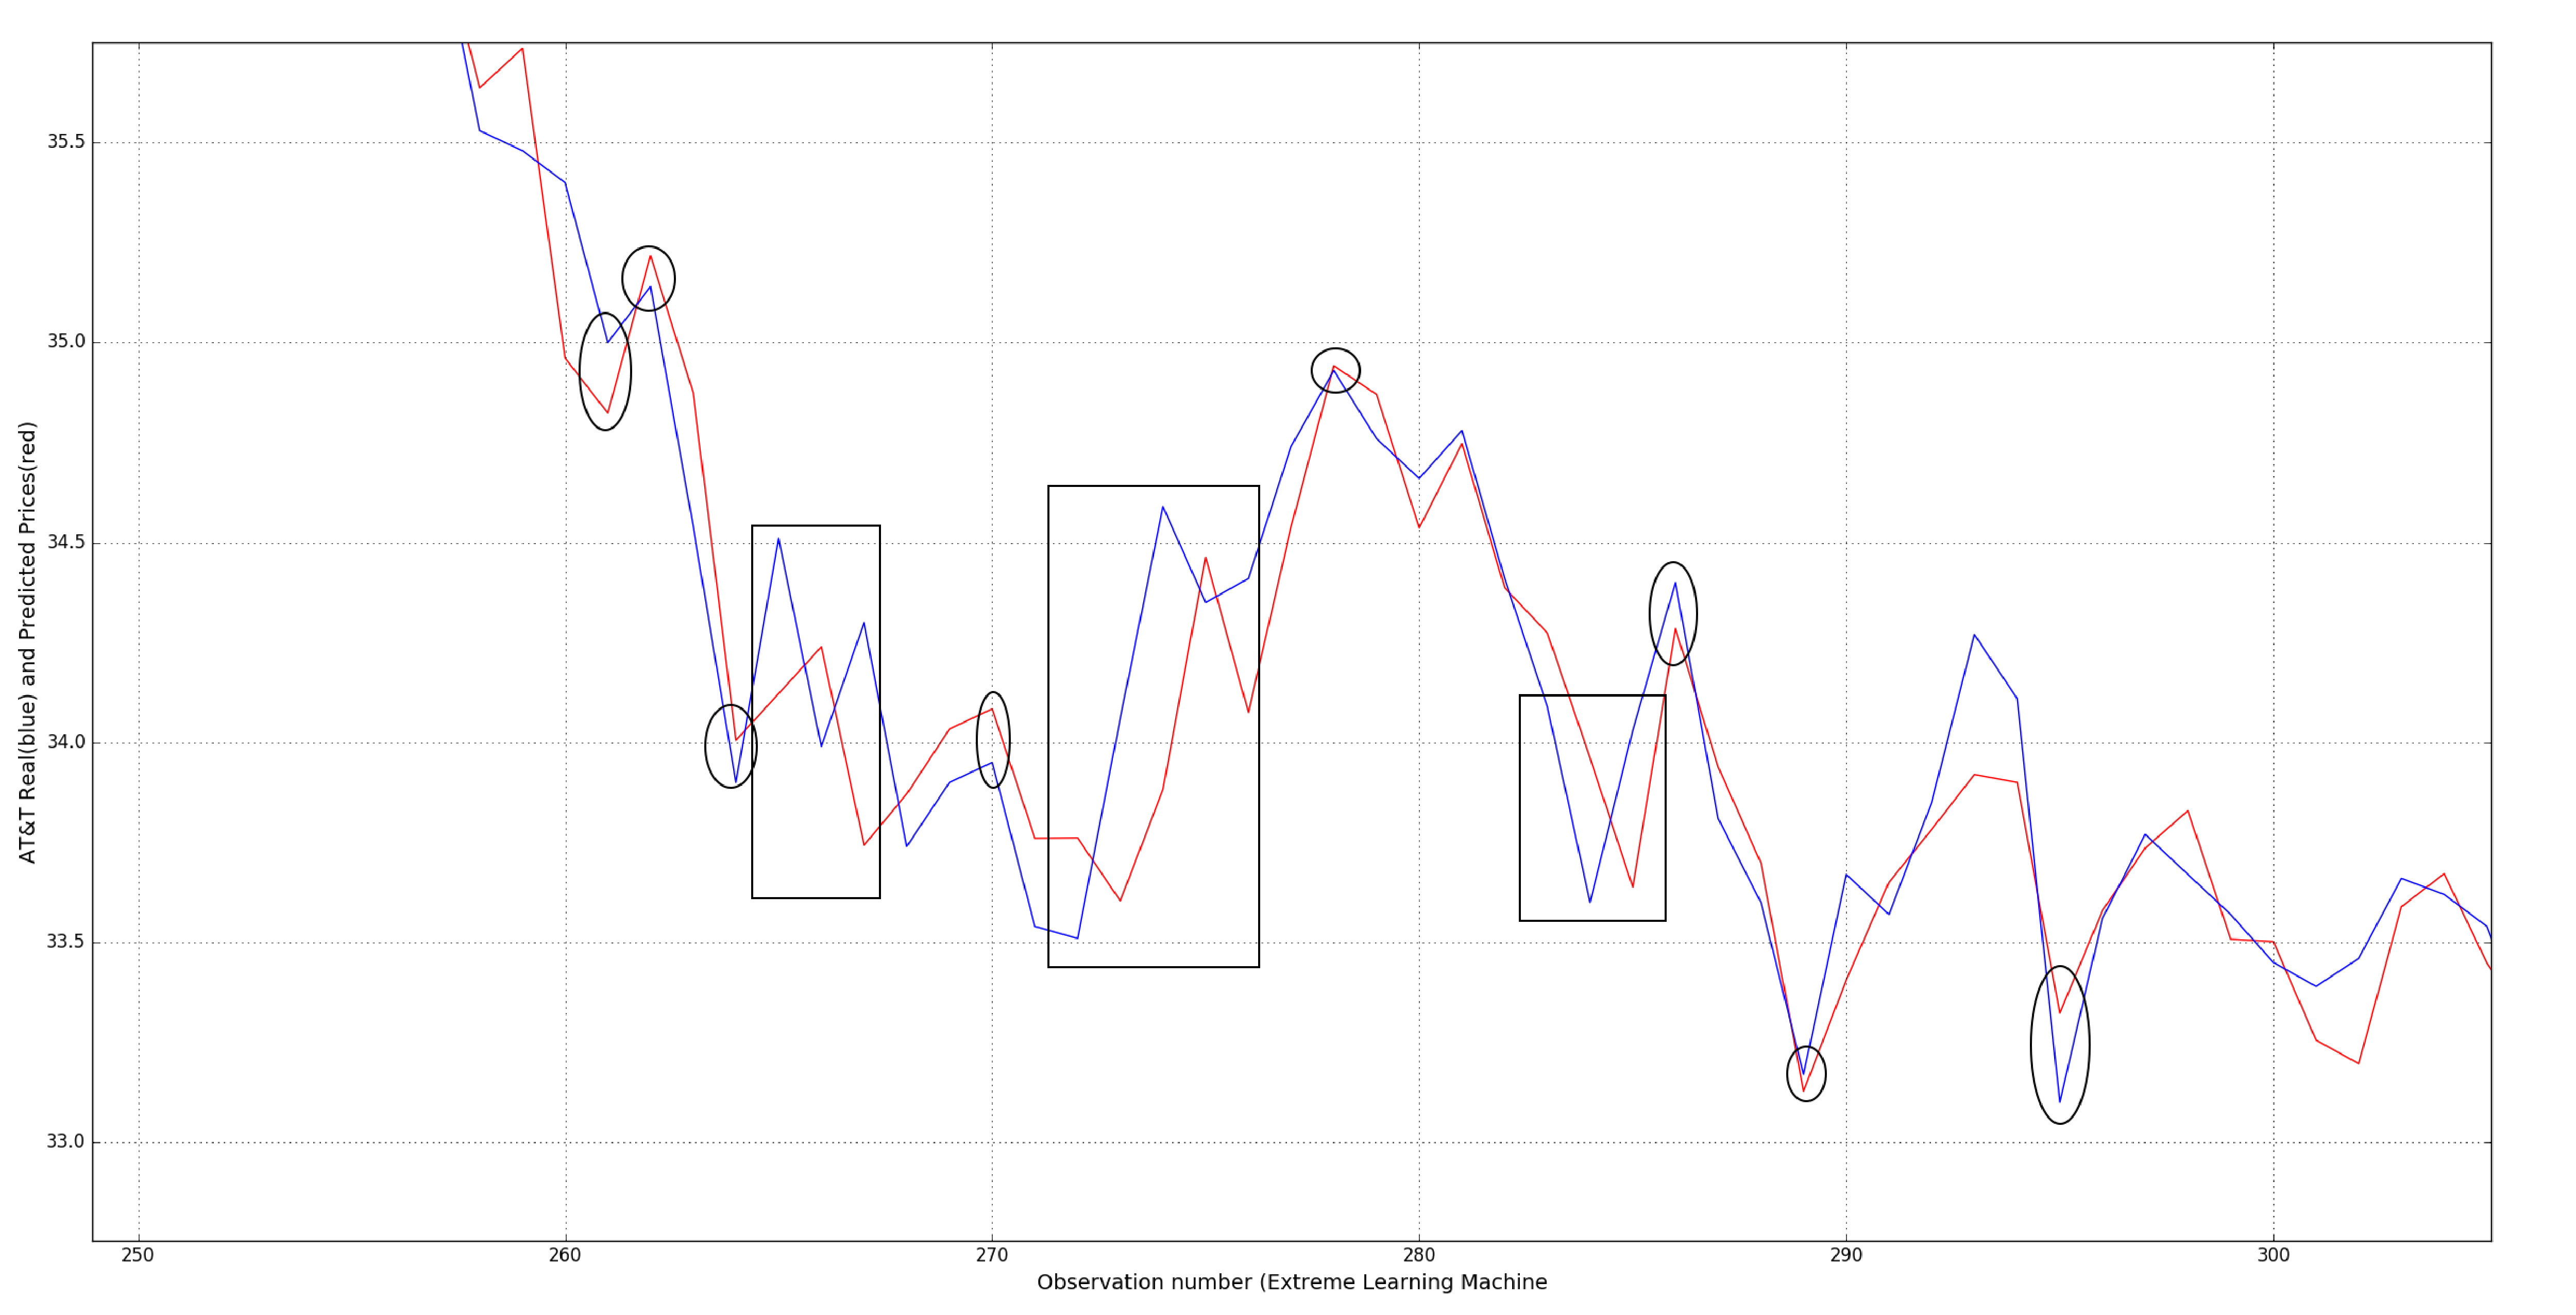
\includegraphics{images/projecting_prices}}
	\caption{ Black Rectangles: Forward Projected forecasts, Black circles: Correct inflection. }
	\label{projected_prices}
	\end{center}
\end{figure}

Projecting data is one of observed patterns that happened for both models.
In this situation, the predicted closing prices (red) look like the forward projection of the real closing prices (blue) within graph~\ref{projected_prices}.
The instances of these projections are outlined with black rectangles.
In these situations, the models found a very simple method of producing a close approximation and lowering the training error, which impacted the results of testing.
The model is reacting to the stock changes instead of reacting with the stock changes.
The graph above was an arbitrary choice, and these patterns were seen infrequently throughout the testing data.

The forward projection of previous closing prices might not be a problem.
Even though both of these models' weights were optimized with different methods, both of these models exhibit this pattern.
This may indicate that the issue is difficult to resolve and is a results of the training process or noisy data.
This could also be a consequence of using Artificial Neural Networks for financial forecasting because neural networks are unpredictable when classifying noisy data.

After projecting previous days forward, both methods were seen to adjust their predictions to correctly forecast inflection points as shown by the black circles.
From the previous section, the Extreme Learning Machine model showed that it predicted the sign of change and inflection points with high accuracy, so on average, the model outperforms the Efficient Market Hypothesis.
The Back-Propagation model was less successful with forecasting the sign of change and inflection points.

\begin{figure}
	\begin{center}
	\resizebox{\textwidth}{!} {
	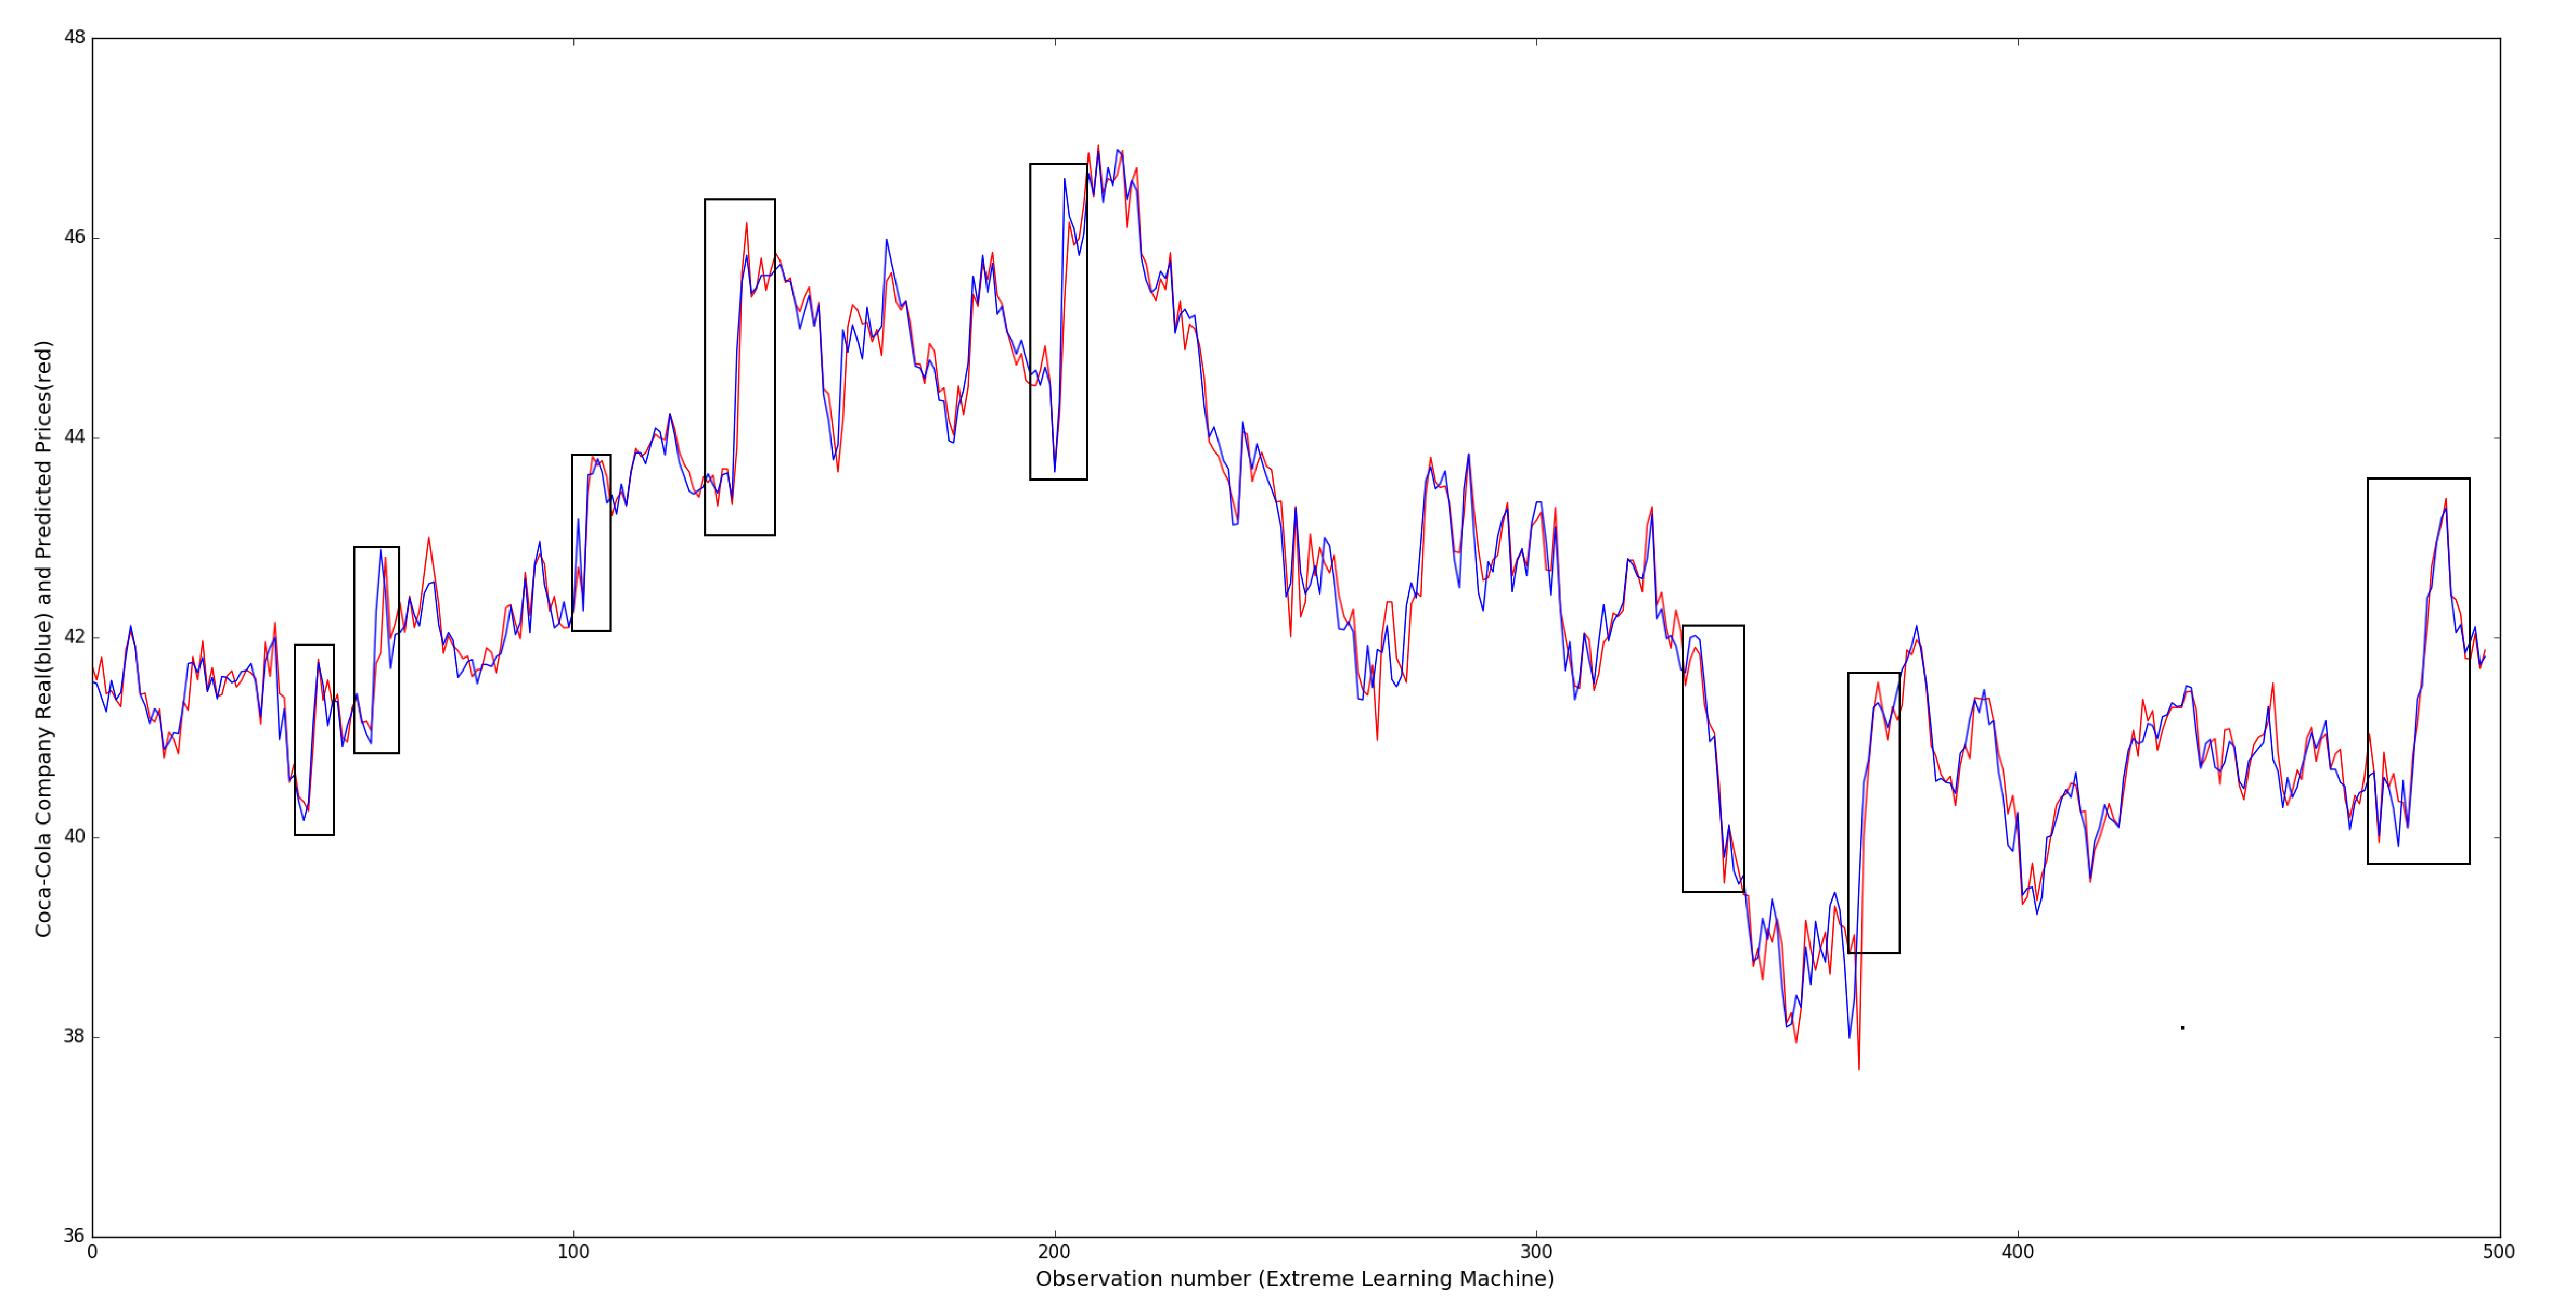
\includegraphics{images/threshold_response}}
	\caption{ Black Rectangles: Forecasted threshold responses }
	\label{threshold_responses}
	\end{center}
\end{figure}

Both models performed well with forecasting threshold responses as in graph~\ref{threshold_responses}.
Thresholds exist in markets where the market begins to quickly change in price.
For the five testing stocks, both models forecasted the same pattern for these rapid price changes.
The Extreme Learning Machine model tended to over predict and under predict these changes less than the Back-Propagation model.
Both models became more proficient at forecasting threshold responses after the data sets were preprocessed using min-max linear scaling.

% Conclusion

	% Conclusion
	\section{Conclusion}\label{sec:conclusion}
	The mathematical theories and methods of training neural networks for forecasting stock markets were presented within this article.
	While the findings of others and this paper have very positive results on independent data, the academic playground mentality might not transfer to an actual financial market.
	If authors modify their testing parameters to perform well on a testing set, then the model might not generalize well to the real world.
	The testing parameters for all of the neural networks were held constant within this experiment with the goal of finding a general model for forecasting daily closing prices.
	The analysis method used only represents half of a larger solution which would scrape new articles, tag parts of speech, rate the article's affect, and factor that new information into forecasts.

	An Artificial Neural Network model represents an important component of a system for forecasting daily stock change.
	Extreme Learning Machines and Back-Propagation with stochastic gradient descent were used and evaluated against each other.
	Of the five different stocks both networks were tested on, the Extreme Learning Machine model had better results.
	The Extreme Learning Machine model had lower training time, lower MSE, and higher classification success.
	The hit or miss ratio provided within this paper implies that Extreme Learning Machines would perform well with forecasting the direction of change in a market.
	Extreme Learning Machines are a relatively new method for optimizing neural networks.
	Another important question to consider is whether Extreme Learning Machines are able to outperform deep learning algorithms.
	More research should be published to further evaluate using Extreme Learning Machines for regression.

	% Acknowledgments
	\section*{Acknowledgments}
	Special thanks to Dr. Miroslaw Mystkowski from the Department of Mathematical Sciences at Gardner-Webb University for his advising and support.

	% References
	\bibliographystyle{apa}
	\bibliography{references}

\end{document}